\section{Design and implementation}
\label{sec:Design}

To overcome the shortcoming of ingress controller, this paper proposes a dynamic load-balancing solution. The solution consists of two part, one part is load monitor, the other part is dynamic load-balancing algorithm.

\subsection{Workflow}
\label{subsec:workflow}
\begin{figure}[htbp]
  \centering
  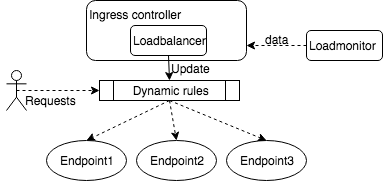
\includegraphics[width=0.45\textwidth]{images/dynamic_solution.png}\\
  \caption{Workflow of dynamic solution}
  \label{fig:dynamic_solution}
\end{figure}
Figure~{\ref{fig:dynamic_solution}} illustrates the workflow of the dynamic load-balancing solution:
\begin{enumerate}[label=(\arabic*)]
  \item Load monitor gather necessary data for dynamic load balancing and offer data to loadbalancer.
  \item Loadbalancer makes a further evaluation for data received from loadmonitor and dispatches incoming requests based on dynamic load-balancing algorithm.
  \end{enumerate}

\subsection{Load monitor}
\label{subsec:load_monitor}

\begin{figure}[htbp]
  \centering
  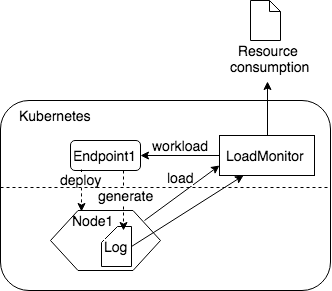
\includegraphics[width=0.45\textwidth]{images/request_learning.png}\\
  \caption{request-learing phase}
  \label{fig:request_learning}
\end{figure}

Load monitor collects, analyzes and outputs information needed by dynamic load-balancing algorithm. Load monitor processes two kinds of information: request logs and endpoint loads.
Request logs are used for evaluating resource consumption of request. Before running in kubernetes, each web service goes through the request-learning phase shown by figure~{\ref{fig:request_learning}}: First, a single endpoint is deployed, then load monitor generates workload by keep on sending requests in a fixed speed to the endpoint, the speed increases with time until it reach the processing limit of endpoint. At the same time, load monitor combines service logs, workload and endpoint load to evaluate resource description for each type of request.
We define $RD_i$ as resource description of  a $i_{st}$ type request.$C_i$ ,$M_i$ and $N_i$ stand for CPU, memory, network consumption to process a $i_{st}$ type request. $S_{i}^{t}$ stands for speed of sending $i_{st}$ type request in timestamp t. $c_{i}^{t}$, $m_{i}^{t}$, $n_{i}^{t}$ are CPU, memory, network load of endpoint in timestamp t during $i_{st}$request-learning phase. The computation of resource description is as follow:

$$ C_i = \frac{\sum_{j=1}^{k}\frac{c_{i}^{t}}{s_{i}^{t}}}{k}, M_i = \frac{\sum_{j=1}^{k}\frac{m_{i}^{t}}{s_{i}^{t}}}{k}, N_i = \frac{\sum_{j=1}^{k}\frac{n_{i}^{t}}{s_{i}^{t}}}{k}$$

$$RD_i = \left \{ C_i, M_i, N_i \right \}$$


Then load monitor enters load-collecting phase shown in figure~{\ref{fig:load_collecting}} to generate load description for endpoints.To increase load-balancing performance, load description of endpoints has to cover all influencing factors. For the resource usage part, Load monitor collects system loads from kubelet, a component that is not only responsible for managing lifecycle of pods, but also takes charge of collecting cluster load. For sharing problem and locality, load monitor obtains endpoint information from apiserver. Endpoint information includes configuration that which endpoints share the same database, which endpoints are deployed in the same node and so on. Table~{\ref{table:load_description}} is an example of load description given by load monitor.
\begin{figure}[htbp]
  \centering
  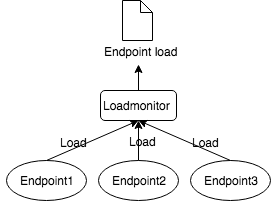
\includegraphics[width=0.45\textwidth]{images/endpoint_load.png}\\
  \caption{load-collecting phase}
  \label{fig:load_collecting}
\end{figure}

\hspace{0pt}
\begin{table}[htbp]
 \begin{center}
  \begin{tabular}{c|c|c|c}
   \hline
   Type           & Pod    & Pod   & Node  \\  \hline
   Name           & App1   & Db1   & Node1 \\ \hline
   CPU limit      & 10     & 10    & 50    \\ \hline
   CPU usage      & 2      & 3     & 20    \\ \hline
   Memory limit   & 100M   & 200M  & 2G    \\ \hline
   Memory usage   & 20M    & 100M  & 500M  \\ \hline
   Network limit  & 1M/s   & 2M/s  & 5M/s  \\ \hline
   Network usage  & 500k/s & 1M/s  & 3M/s  \\ \hline
   Node           & Node1  & Node1 & -     \\ \hline
   Database limit & Db1    & -     & -     \\ \hline
  \end{tabular}
 \end{center}
 \caption{Load description}
 \label{table:load_description}
\end{table}



\subsection{Dynamic load-balancing algorithm}
\label{subsec:algorithm}

The dynamic load-balancing algorithm considers request consumption and endpoint load to even workload across endpoints. It aims to reduce overload endpoints and promote RPS. The algorithm is divided into two phase: Classification phase and dispatching phase.
During classification phase, we evaluate requirement of requests, utilization of nodes and ability of endpoints and classify them. For evaluating requests, we let requests compare with each other to get their consumption level of CPU, memory and network, that is to know whether their consumption is high or not compared to others. For evaluating node, we simply adopt utilization rate under the assumption that hardware configuration of all nodes in kubernetes are the same. For the pod part, first we compare usage of CPU, memory and network among pods to get their load level, then we take load level, utilization rate and ability of node and database that pods rely on in to consideration to evaluate ability of endpoints. The evaluation is as follow:
\begin{enumerate}
 \item Calculate requirement level of each request type in CPU, memory and network:
       $$L_{max} = Max\left \{ L\_f_1,...,L\_f_i \right \}$$
       $$L_{min} = Min\left \{ L\_f_1,...,L\_f_i \right \}$$
       $$r\_f_i =  \frac{L\_f_i - L_{min}}{L_{max} - L_{min}} \cdot 100\%$$
       $$R\_f_i=\left\{
       \begin{matrix}
        High & r\_f_i\geq T_r \\
        low  & r\_f_i < T_r
       \end{matrix}
       \right.$$
       where $L\_f_i$ is consumption of a given factor among CPU, memory and network, $r\_f_i$ represents consumption of  $i_{st}$ request type among all request types.$R\_f_i$ is requirement level. For each request type, its requirement is $\left \{ R\_CPU, R\_MEM, R\_NET \right\}$. By default, we set the threshold $T_r = 0.5$.

 \item Calculate utilization of node in CPU, memory and network:
       $$U_i = \frac{{L\_usage}_i}{{L\_limit}_i} \cdot 100\%$$


       where $L\_usage_i$ and $L\_limit_i$ denote usage and limit of a given factor among CPU, memory and network, $U_i$ represents utilization of $i_{st}$ node.For each node, its utilization is $\left \{U\_CPU, U\_MEM, U\_NET\right\}$.

 \item Calculate ability of pod in CPU, memory and network:
       $$L_{max} = Max\left \{ L\_usage_1,...,L\_usage_i \right \}$$
       $$L_{min} = Min\left \{ L\_usage_1,...,L\_usage_i \right \}$$
       $$U_i = \frac{{L\_usage}_i}{{L\_limit}_i} \cdot 100\%$$
       $$P_i = \frac{L_\_usage_i - L_{min}}{L_{max} - L_{min}} \cdot 100\%$$
       $$A_i = 1- \left ( U_i \cdot \alpha + P_i \cdot \beta + N_i \cdot \gamma + D_i \cdot \delta\right )$$
       $$\left ( \alpha + \beta + \gamma + \delta = 1 \right ) $$

       where $L\_usage_i$ denotes usage of a given factor, $L\_limit_i$ is the limit, $U_i$ stands for utilization rate, $P_i$ represents load level, $N_i$ and $D_i$ are utilization of node and ability of database that  pod relies on. For database pods, the $D_i$ is zero.By default, we set $\alpha = 0.5, \beta = 0.1, \gamma = 0.2, \delta = 0.2$. For each pod, its ability is $\left \{A\_CPU, A\_MEM, A\_NET\right\}$.
\end{enumerate}

During dispatching phase, endpoints are sequenced by their ability: Firstly, we set up thresholds to group endpoints. That is $T_{c} = 70\%$ for deciding whether endpoint's CPU ability is in high or normal level, $T_{m} = 50\%$ for deciding whether endpoint's memory ability is high or normal, $T_{n} = 50\%$ for deciding whether endpoint's network ability is high or normal. As a result, endpoints are grouped into 8 groups. Table~{\ref{table:endpoint_groups}} shows definition of these groups.

\hspace{0pt}
\begin{table}[htbp]
 \begin{center}
  \begin{tabular}{c|c|c|c}
   \hline
   Group & CPU               & Memory            & Network           \\  \hline
   g1    & $A\_CPU \geq T_c$ & $A\_MEM \geq T_m$ & $A\_NET \geq T_n$ \\ \hline
   g2    & $A\_CPU \geq T_c$ & $A\_MEM \geq T_m$ & $A\_NET < T_n$    \\ \hline
   g3    & $A\_CPU \geq T_c$ & $A\_MEM < T_m$    & $A\_NET \geq T_n$ \\ \hline
   g4    & $A\_CPU \geq T_c$ & $A\_MEM < T_m$    & $A\_NET < T_n$    \\ \hline
   g5    & $A\_CPU < T_c$    & $A\_MEM \geq T_m$ & $A\_NET \geq T_n$ \\ \hline
   g6    & $A\_CPU < T_c$    & $A\_MEM \geq T_m$ & $A\_NET < T_n$    \\ \hline
   g7    & $A\_CPU < T_c$    & $A\_MEM < T_m$    & $A\_NET \geq T_n$ \\ \hline
   g8    & $A\_CPU < T_c$    & $A\_MEM < T_m$    & $A\_NET < T_n$    \\ \hline
  \end{tabular}
 \end{center}
 \caption{Endpoint groups}
 \label{table:endpoint_groups}
\end{table}

A new endpoint is inserted into a desired group by insertion sort algorithm in descending order first by A\_CPU, then A\_MEM and finally A\_NET.  The  algorithm~{\ref{alg:insertion}} describes the insertion.

\begin{algorithm}
 \caption{modified insertion sort algorithm}
 \label{alg:insertion}
 \begin{algorithmic}[1]
  \Require $g\left [\right]$, $endpoint$
  \State $i \gets 0$
  \While{$i<sizeof\left (g\right)}$}
  \If {$ !\left(endpoint.A\_CPU \geq g\left [i\right].A\_CPU\right)$\textbf{and}\\  $\left(endpoint.A\_MEM \geq g\left [i\right].A\_MEM \right)$}
  \State $i++$
  \State continue
  \ElsIf {$endpoint.A\_CPU \geq g\left [i\right].A\_CPU$}
  \State break
  \EndIf
  \State i++
  \EndWhile
  \State \Call {Do\_insertion}{$g,i,endpoint$}
 \end{algorithmic}
\end{algorithm}
\begin{algorithm}
 \caption{selection algorithm}
 \label{alg:choice}
 \begin{algorithmic}[1]
  \Require $hg\left [ \left \{ ep\, | ep\, \,\epsilon \, g1\cup g2\cup g3\cup g5  \right \} \right ]$,

  $lg\left [ \left \{ ep\, | ep\, \,\epsilon \, g4\cup g6\cup g7\cup g8  \right \} \right ]$,$request$
  \Function{random\_choice}{hg,lg}
  \If {$sizeof\left(hg\right) == 0$}
  \If {$sizeof\left ( lg \right )\leq 3$}
  \State \Return {$lg$}
  \Else
  \State $i,j,k = \Call {random\_3int}{0,sizeof\left(lg\right)}$
  \State \Return $\left \{ lg\left [ i \right ] ,lg\left [ j \right ] ,lg\left [ k \right ] \right \}$
  \EndIf
  \ElsIf{$sizeof\left ( hg \right )\leq 3$}
  \State \Return {$hg$}
  \Else
  \State $i,j,k = \Call {random\_3int} {0,sizeof\left(hg\right)}$
  \State \Return $\left \{ hg\left [ i \right ] ,hg\left [ j \right ] ,hg\left [ k \right ] \right \}$
  \EndIf
  \EndFunction
  \Function{scorecandidate}{candidate,request}
  \State $i \gets 0$
  \While {$i<sizeof\left(candidate\right)$}
  \State $S\_c \gets candidate\left(i\right).A\_CPU \ast request.\theta$
  \State $S\_m \gets candidate\left(i\right).A\_MEM \ast request.\lambda$
  \State $S\_n \gets candidate\left(i\right).A\_NET \ast request.\mu$
  \State $candidate\left(i\right).Score = S\_c+S\_m+S\_n$
  \EndWhile
  \State $\Call {sortbyscore}{candidate}$
  \State \Return $candidate$
  \EndFunction
  \State $c \gets \Call{random\_choice}{hg,lg}$
  \State $c \gets \Call {scorecandidate}{c}$
  \If {$request.priority == High$}
  \State $\Call {dispatch\_request}{request,highestof\left(c\right)}$
  \Else
  \State $\Call {dispatch\_request}{request,middleof\left(c\right)}$
  \EndIf
 \end{algorithmic}
\end{algorithm}
The dispatch decision is made based on request requirement level and endpoint groups. The steps of dispatching a request is as follow:
\begin{enumerate}
 \item Query request type and corresponding requirement level.

 \item Select suitable endpoint for request, the selection is decided by selection algorithm~{\ref{alg:choice}}. First of all, we define priority of endpoint groups: we regard g4,g6,g7,g8 as low-priority groups and g1,g2,g3,g5 as high-priority groups because of the fact that endpoints have poor performance when they score badly in more than one factor. Then we pick three endpoints as candidates randomly from high-priority groups, grade them and choose the most suitable one. The equation to grade endpoints is as follow:
       $$G_i = A\_CPU_i \cdot \theta + A\_MEM_i \cdot \lambda + A\_NET \cdot \mu$$
       $$\theta + \lambda + \mu = 1$$
       Where $G_i$ is score of $i_{st}$ endpoint. Especially, selection is performed independently between high-priority and low-priority groups, if there is no endpoint in expected priority groups, we make the selection among other priority groups, if there are one or two endpoints, we simply choose all of them as candidates without picking more endpoints from other priority groups. After grading candidates, we have a highest-scored endpoint, a middle-scored and a lowest-scored endpoint. For candidate set with one endpoint, the highest-scored, the middle-scored and the lowest-scored endpoint are the same one. For candidate set with two endpoint, the middle-scored and the lowest-scored endpoint are the same one. Then we define priority of request: we regard requests whose requirement level ranks high in at least two factor as high-priority requests, we regard the others as low-priority requests. Based on request priority, we have different values for $\theta, \lambda, \mu$, and different selecting strategy. Table~{\ref{table:request_priority}} describes the definition of request priority.
       Table~{\ref{table:selecting_strategy}} gives a hint to select candidate for different request priority.
       High-priority requests consume more resource than others, so we choose the highest-scored candidate for them.
       As for low-priority requests, we choose middle-scored one instead. In this way, we use middle-scored candidates which are healthy enough to
       handle low-priority requests to reduce workload of high-scored candidates to prevent the situation that high-scored candidate become
       overhead quickly because requests of all priority rush to them.
       \hspace{0pt}
       \begin{table}[htbp]
        \begin{center}
         \begin{tabular}{c|c|c|c|c}
          \hline
          Type     & CPU  & Memory & Network & Priority \\ \hline
          request1 & High & High   & High    & High     \\ \hline
          request2 & High & High   & Low     & High     \\ \hline
          request3 & High & Low    & High    & High     \\ \hline
          request4 & High & Low    & Low     & Low      \\ \hline
          request5 & Low  & High   & High    & High     \\ \hline
          request6 & Low  & High   & Low     & Low      \\ \hline
          request7 & Low  & Low    & High    & Low      \\ \hline
          request8 & Low  & Low    & Low     & Low      \\ \hline
         \end{tabular}
        \end{center}
        \caption{request priority}
        \label{table:request_priority}
       \end{table}

       \hspace{0pt}
       \begin{table}[htbp]
        \begin{center}
         \begin{tabular}{c|c|c|c|c}
          \hline
          Type     & $\theta$ & $\lambda$ & $\mu$ & Selected endpoint \\ \hline
          request1 & 0.4      & 0.3       & 0.3   & highest-scored    \\ \hline
          request2 & 0.4      & 0.4       & 0.2   & highest-scored    \\ \hline
          request3 & 0.4      & 0.2       & 0.4   & highest-scored    \\ \hline
          request4 & 0.6      & 0.2       & 0.2   & middle-scored     \\ \hline
          request5 & 0.2      & 0.4       & 0.4   & highest-scored    \\ \hline
          request6 & 0.2      & 0.6       & 0.2   & middle-scored     \\ \hline
          request7 & 0.2      & 0.2       & 0.6   & middle-scored     \\ \hline
          request8 & 0.4      & 0.3       & 0.3   & middle-scored     \\ \hline
         \end{tabular}
        \end{center}
        \caption{selecting strategy}
        \label{table:selecting_strategy}
       \end{table}
 \item Rewrite destination of request with the selected endpoint IP and dispatch request.
\end{enumerate}

It is worth mentioning that the algorithm is based on dynamic data provided by load monitor except for
request data. The resource consumption, which is a static and stable property of request, is seemed to remain almost the same for a rather long time,
so we just evaluate it for once in load monitor. As for dynamic system load of nodes and endpoints, load monitor keeps on collecting load all the time and
reports them to loadbalancer at intervals.Loadbalancer makes load-balancing decision based on the newest verison of data it received from load monitor until
the next interval arrives. The length of interval has a great influence on the overhead and performance of loadbalancer. Whenever a new interval time arrives,
loadbalancer has to recompute the endpoint load to get real-time load so with the increasement of interval, it costs less overhead to compute but has worse
performance because the load are not real-time enough. We set the interval to 5 second to make a trade-off between performance and overhead.
